\chapter{Analysis}

This chapter describes the considerations taken in picking an algorithm, as well as what is already implemented at Infomedia.

\section{Algorithms in General}
Before any sort of work can be done, one must consider various algorithm to work with. There are several text matching algorithms available for free on the Internet, and if one has the money for it, there are companies that can develop a specialized algorithm for you. As I do not have a lot of money (and paying for someone else, to do an algorithm for me, kind of defeats the purpose of this whole thesis) I have gone with the first option and found a free basic algorithm on the Internet, as well as contemplated to create my own algorithm from scratch.

\subsection{Requirements Analysis}
The algorithms should be able to live up to the following demands:

\begin{itemize}
	\item The algorithm should be able to work with text.
	\item Performance is of secondary importance, but should have good accuracy (performance < accuracy).
	\item The algorithm shall be able to return a score based on how identical two articles are.
	\item The algorithm should be focus on doing one thing only (not try to do several forms of text comparisons).
	\item The algorithm shall be available in an open source, or free to use, licence.
\end{itemize}

\section{Initial Considerations}
Infomedia already have an algorithm implemented in the inflow to make a rough comparison of the articles coming in. How ever, the thought is that a combination of several algorithms would provide a better and more granular view of the articles as they are being compared. A new algorithm should be one that was specialized in text matching. It should also be an algorithm that would work in different manner than what Infomedia already have implemented\footnote{More on the algorithm already implemented in the next section.}, as having two algorithms that work in more or less the same fashion would not produce results of much interest.

As the current implementation is rather fast, it could prove useful to have the algorithm that is already implemented, do the initial rough split of matches and no matches, and then have a slower (but more thorough) algorithm look at the \textit{interesting} article comparisons. Initially I have looked at two algorithms to fill this need, \textit{Longest Common Substring} and \textit{Semaphore Tag Matching} - an algorithm I would make from scratch.

\subsection{System Architecture}
As mentioned the various algorithms should work in different ways, meaning they should have various ways. This is to ensure a balanced image of how much an article comparison is actually a match. The thought is, that instead of having a few algorithm having to have many focus areas. It is better to have many that only focus on one thing, then combine their scores into a broad representation of how similar two articles is.

\pagebreak

\begin{figure}
	\centering
	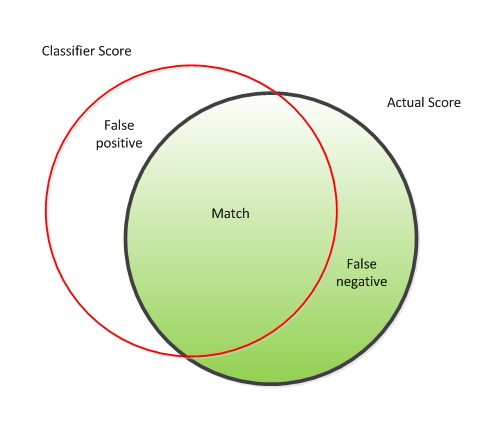
\includegraphics[scale=0.5]{figures/SingleAlgoScore}
	\caption{Variation between how a single algorithm might score an article comparison, and how the actual score should be\cite{Slides}.}
\end{figure}

The essential thing in this, is to ensure that the various algorithms works in different ways. If one were to use many algorithms that all focused on the same way of doing text comparisons, the results would not provide that broad image of scores that is wanted for a more accurate score representation.

\begin{figure}
	\centering
	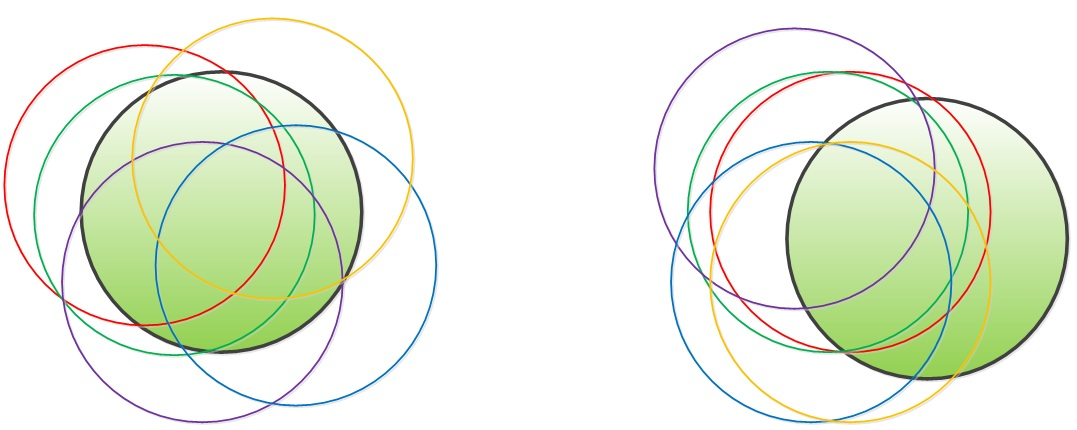
\includegraphics[scale=0.3]{figures/MultipleAlgoScores}
	\caption{\textbf{Left:} A balanced score, obtained by using several algorithm with different focus areas. \textbf{Right:} An unbalanced score, obtained by using several algorithms with the same focus area\cite{Slides}.}
	\label{MultipleAlgo}
\end{figure}

The idea is that the algorithms should do 99.9\% of the work in identifying article duplicates, and then have the  last 0.1\% be verified by humans. This is already how things are working at Infomedia, but only with one algorithm at the moment. My work will the be the first algorithm to do a check of the work done by the already implemented algorithm. This will hopefully narrow the field of possible article duplicates that has to be verified by human eyes.

The system would then ideally work as follows.

\begin{figure}[h]
	\centering
	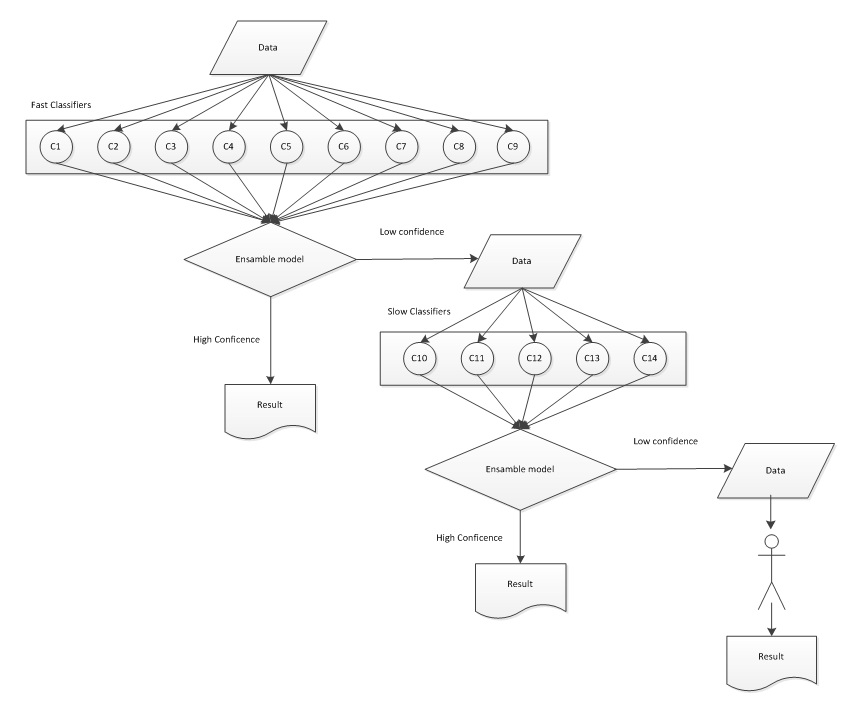
\includegraphics[scale=0.5]{figures/SystemArchitecture}
	\caption{System Architecture, with many algorithms doing text analysis\cite{Slides}.}
	\label{Architecture}
\end{figure}

When data (articles) arrives in the inflow, a number of fast algorithms would then do the rough split of the comparisons. All of these comparisons would then receive scores, that would then be evaluated through the ensemble model. If the scores leaves no doubt (is over a given threshold) that the article comparison is a match, the comparison would stored as a match. If the scores of the comparisons leaves some degree of doubt as to whether a comparison is a match or not (the scores being between a set of thresholds), the comparisons are then passed on to the slower algorithms, that then in turn would evaluate the comparisons. If these algorithms find that the comparison is a match, it would be stored as such. If there is still some doubt to whether it is a match or not, the articles would then finally be sent for human evaluation. 
The task of my thesis is to create a secondary algorithm (one of the slower ones) to evaluate the results given from the faster (and already implemented) algorithm.

\section{Algorithms Used}

\textbf{Term Frequency - Inverse Document Frequency\cite{WikiTFIDF} (Cosine)}, generates a vector from each document. \textbf{I will not cover this algorithm in detail, as I have not done any work on it, only used some of the methods in it for my thesis.} This is the algorithm already implemented in the inflow today (a modified version of it, that is based on the Vector Space Model\footnote{\url{http://en.wikipedia.org/wiki/Vector_space_model}}). Each word in every article is added to a \textit{word map} which contains all the words of all articles in the corpus being checked (which also is used to create the document vector). The word map is used to generate a weight of each word (a word occurring in many articles will have less weight than a word that is only present in a few articles). Each word generates a bit of the articles total vector, a word that occurs in all documents will have a very short vector, a more rare word will have a longer (and therefore weigh heavier) in the article vector.

Once the word map is created, the articles are then scored. The way that this is done, is that the algorithm compares two article's vectors with each other and then returns a score based on the cosine angle between the two article vectors. This is done one article comparison at a time (although done with parallel coding to speed up the process). As the word map is generated each time the algorithm is run, the word map can (and probably will) differ from each run (if the corpus of articles are being changed). Infomedia is therefore talking about implementing this bit differently, and building a constant word map, that only gets updated with each run, not overwritten. This will ensure that common words will always have a short vector.

The algorithm then returns a list of article comparisons (based on a threshold set by the user), with article ID\footnote{Each article has their own unique ID.} and scores. So each comparison has the ID of \textit{"article 1"} and \textit{"article 2"} and their score (the angle between the two vectors, in a multidimensional universe). The closer the score is to the value 1.0 the more similar are two articles. A score of 0.0 indicates that two articles has nothing in common (according to this algorithm, I will discuss this point in the next paragraph), whereas a score of 1.0 indicates two perfectly identical articles (according to this algorithm). This algorithm and it has a good O-notation (O(log N)).

\textbf{Problem:} \label{CosineProblem} This string comparison is very sensitive to articles containing many of the same words, for instance "A man walks his dog in the park" and "A dog walks his man in the park" would result in returning a cosine value of 1.0, due to the way the algorithm works. The two strings are clearly different, but the words in each string is the same, therefore the Cosine algorithm will find them to be identical. This problem is very unlikely to yield false positives.

\textbf{Longest Common Substring (LCS)}, compares documents in pairs. A general implementation would be to have a list of documents and then compare a document to every other document in the list. The algorithm will then return the length of the longest common substring. By default the LCS algorithm\cite{WikiLCS} checks the contents of a string character by character against another string. When initialized, the algorithm creates an double array and each time a match is found (when two identical characters are found ('a' and 'a' for instance)) the algorithm marks that in the array by adding a number. It then checks if this substring is longer than what has previous been found, if so, it discards the old substring and keeps the newly found.

\begin{figure}[h]
	\centering
	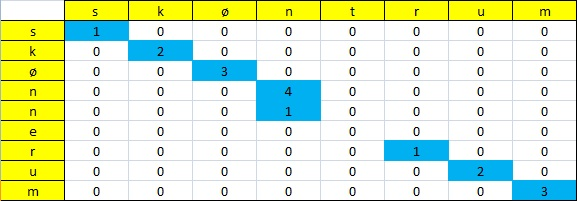
\includegraphics[scale=0.75]{figures/LcsExplained}
	\caption{An example of how two words are compared in LCS. The fields in yellow are the two words broken into characters ('Skøntrum' and 'Skønnerum'). The fields in blue indicates when LCS finds a match, the number indicates the length of the substring. In this case, LCS finds three sub strings:'skøn', 'n' and 'rum', the longest of the three is the first, and this will be the result that LCS returns to the user. }
	\label{LcsExplained}
\end{figure}

I will use the basic implementation of this algorithm in my thesis, I will then try and modify it to work better in context with finding article duplicates, instead of just the longest common substring.

\textbf{Problem:} This algorithm is very prone to fail in cases where there have been made alterations to the article in question. A word change in the middle of one of two otherwise identical articles will result in a ~50 \% match. If the article in question have been obfuscated with many changed words, the LCS will be extremely short. This is a high risk problem, as article duplication will often involve changing words. This algorithm is also substantially slower than the Cosine algorithm, having an O-notation of O(n*m). Ideally this algorithm is therefore best used on a selection of articles, rather than on the entire corpus.


\section{Optimizing Performance}
\subsection{Stop Words}
Stop word\footnote{\url{http://en.wikipedia.org/wiki/Stop_words}} removal would improve running time (performance) of both algorithms, and would pose little threat of causing either algorithm to fail (finding false positives). The exception to this could be very short articles (like breaking news articles\footnote{Breaking News articles is a thing of the 2000s. With the spread of media onto the Internet, an article is no longer a static printed piece of news in a paper. News can be published instantly on the web, and then updated as information are received. How ever, Breaking News articles can still be printed in the paper article with only little text attached to it.}), that only contains common words, like "Man walks away". Depending on the stop word list, this article could end up being \textit{null\footnote{An article with no text data.}}.
We can safely (with respects to the previously addressed problem) remove stop words, as they don't provide any \textit{semantic\footnote{\url{http://en.wikipedia.org/wiki/Semantics}}} value to the text.

\subsubsection{Cosine}
For the cosine algorithm removal of stop words would improve performance, by reducing the size of the \textit{Magnitude Vector}. 

\subsubsection{LCS}
In regards to the LCS algorithm, the performance would also be improved, as the algorithm wouldn't need to traverse as many characters. This would reduce the length of the longest common substring, but it would be unlikely that it would affect the outcome of the algorithm, as stop words are rarely changed when duplicating articles.

\subsection{Stemming}
\textit{Stemming}\footnote{\url{http://en.wikipedia.org/wiki/Stemming}} Stemming is the act of conjugating a word to the base form (Danish:\textit{'Grundform'}). It is done in order to reduce the amount of noise in a text. Words will then be conjugated and instead of having the same word represented several time in different conjugations they will all be noted as the same word. Stemming does not ruin the semantic content of the text.

\subsubsection{Cosine}
Stemming improves the performance of the cosine algorithm as this will reduce the number of words in the \textit{vector space}. As words would be reduced to their base form (Danish:\textit{Grundform}), words used several times, but with different endings would be counted as the same word. When using weighed evaluation this would actually improve performance to some extend. It can have a slight impact of the Cosine algorithm. This is because that without stemming the same word can occur several times in a text in different conjugations, and thus each conjugation would have a larger vector than when the conjugations are all counted as the same word. This impact will be minimal because the rare words are still occurring less often than normal words (stop words).

\subsubsection{LCS}
Stemming would not improve the performance of the LCS algorithm by much. As this algorithm matches characters one by one, it would make little difference if the words are stemmed or not. As the 'Grundform' is the shortest form of a word in Danish, it will make a slight difference, but this is hardly worth noting.

\section{Semaphore Tagging}
Another way of finding duplicates is by looking at each articles semaphore tags. When Infomedia receives articles in the inflow, these articles are enriched with \textit{Semaphore Tags}\footnote{Semaphore tags are tags that describes the contents of the article, an article about financial fraud would contain the tag \textit{Economic Crime}. These tags are created by the Infomedia Ontology (\url{http://en.wikipedia.org/wiki/Ontology_(information_science)}) team. They are creating rules for when a certain word (or words) appear in certain context, then an article will be tagged with a certain semaphore tag.}. A tag also has relations to other tags. A politician would be tagged with politics, political party, other people in politics that are in some way associated with that person. The tag is also enriched with a score, that is based on the relevance for that tag in that given article. So if a politician is the main focus of an article, the name of that politician is high than if the article deals with something that the politician only have a remote connection to. Each article then gets a number of tags based on what terms are found in the article. A way of finding article duplicates could be through creating an algorithm that would check a pair of articles with their respective semaphore tags.

\subsection{Cons to Semaphore}
As these tags are more of a general indicator to an articles' contents than an actual text matching algorithm, it will provide very little value as a stand alone implementation. Each article will only contain tags for the terms, for which the ontology team has created semantic rules for. If 100 articles all contained various doings of a minister (picking up the children, going to meetings, being involved in a crisis) many of the same tags would be present in the 100 articles, this could be the ministers name, political party and other general tags that are linked to this minister. It would therefore be hard to decipher much information that could truly and uniquely link two articles together just by doing this. However this could be used to enhance another algorithm (for instance one of the two mentioned above). If the articles compared contains the same tags, they are likely to have some sort of relevance to each other, and if the tags also have matching scores, that would strengthen the possibility of a match. I will not look any further into implementing this algorithm in this thesis, as this approach is difficult in providing a definite result.

\section{Text Preparation}
\label{TextPrep}
To reduce the chance of the algorithms failing in detecting duplicates, the text should be 'normalized'. As there are quite a few pitfalls in text analysis, one should try and take as many precautions as possible. A common source of error is common spelling errors, I will not check my article for spelling errors. These can have a rather big impact on the LCS algorithm. However as all text editors today have spell checking, this will be a tiny error source.

As the focus of this thesis have been on proving the thesis statement, there has been done no text preparation other than what is already implemented.

Another problem with text analysis is localized spelling. An example of this can be the Swedish town of Malmö. The issue here being the 'ö' letter which is in the Swedish alphabet. This town's name can be spelled in a few different ways.


\begin{itemize}
\item Malmö (Swedish spelling)
\item Malmø (Danish and Norwegian spelling)
\item Malmo (English spelling)
\item Malmoe (Phonetic spelling of the 'ö' character)
\end{itemize}

The same article could be in different newspapers, but with different spelling of the word. All words, or rather words containing special characters (non English characters) should therefore be normalized. In this case, the character 'ö' could be normalized into the letter 'o'. The phonetic spelling of the 'ö' character is highly unlikely to occur, as the normalized way of spelling 'Malmö' in languages without the 'ö' vowel, would be the third option. There is a lot of issues in this regard. This could be words or characters in a non Latin alphabet (Cyrillic, Arabic, Greek letters used in SI references or others). For this thesis, there is few non Danish texts or words in the test corpus, so it will have little influence. I will in this thesis not normalize text, but accept that minor deviance in scores can occur due to this.

Another good choice in text preparations is to lower case and remove all non alpha numerical characters. This can be advantageous for instance when looking at the name of the current Danish prime minister, Helle Thorning-Schmidt. As the hyphen can often be forgotten the last name can easily be misspelled. Removing the hyphen and replacing it with a blank space character would improve the accuracy of the algorithms. 

Stemming is another good way of normalizing text, I have already covered this topic in a previous section, and will not cover this more in detail here. 

Stop words will reduce the number of words in an article, and with less words, there are less error margin in terms of spelling errors, also less words in the article text means less words that has to be analysed. As stop words have little meaning when trying to figure out if two articles match, it is a good idea to remove these in order to improve performance. 

Unfortunately due to the time limit of this thesis, I will not be able to look into any of text the preparations mentioned, but wanted to describe what should be kept in mind, when implementing this project into Infomedia's inflow.

Finally it is important that all files are stored with the same encoding\footnote{\url{http://en.wikipedia.org/wiki/Character_encoding}}, as different encoding could cause havoc in the systems ability to read the text in the files. This is already done in the system, so I will not worry about this factor in my thesis.

\section{Technology}
As the inflow system at Infomedia is created in C$^\sharp$, it is the easy (and logical) choice to create my work in C$^\sharp$ as well. This would help integrating my work into the existing systems without too much trouble. I am using Visual Studio 2013 and .NET version 4.5 for my code development, which is provided to me by Infomedia. I am using Infomedias Team Foundation Server (TFS) for version control. 








